%!TEX root = ../main.tex

\vspace{-1em}

% =================================================

\section{\color{red}Deformation and Motion}

% =================================================

\begin{Figure}
    \center{
    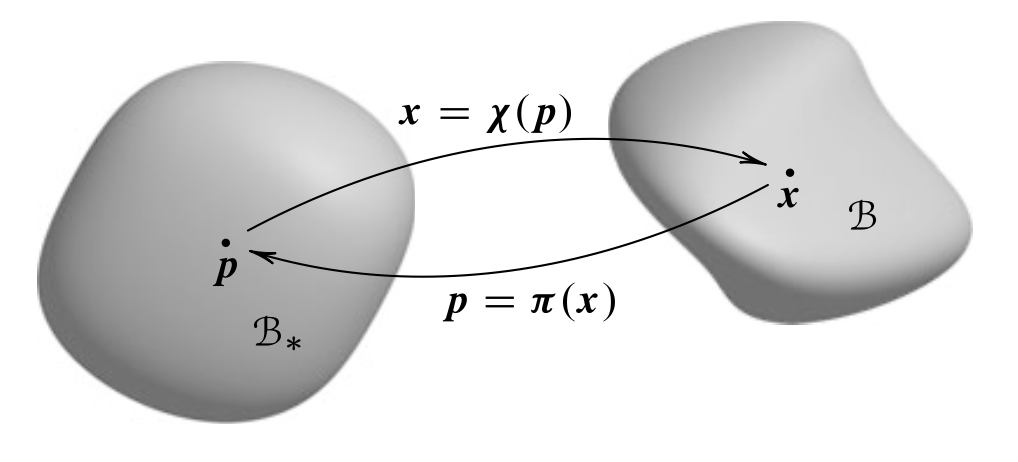
\includegraphics[width=0.8\linewidth]{images/def0}\ \ }
\end{Figure}

\textbf{Deformation gradient.} $F(p)=\nabla_{\!p}\chi$ such that
\begin{equation*}
\chi(q)=\chi(p)+F(p)[q-p]+o(q-p)
\end{equation*}

Fix origin and coordinate axes, $\de \underline{x}=F\,\de\underline{X}$ and component-wise it is
\begin{equation*}
F_{iK}=\frac{\partial x_i}{\partial X_K} 
\end{equation*}

Moreover, F can be seen as a linear trasformation
\begin{equation*}
F:T_{_X} \bt_*\to T_x \bt
\end{equation*}

\begin{Figure}
    \center{
    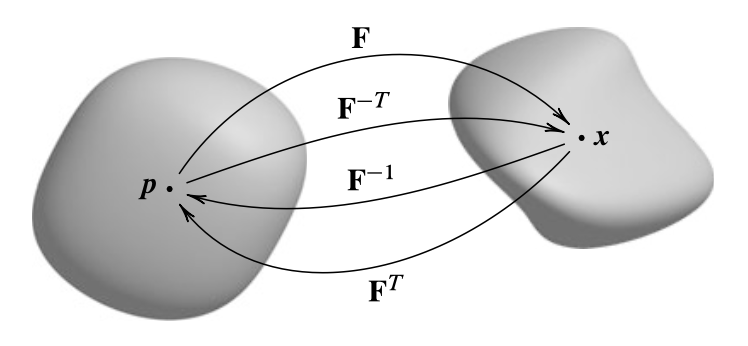
\includegraphics[width=0.7\linewidth]{images/def1}\ \ }
\end{Figure}

\rule{0.31\textwidth}{0.2pt}
\smallskip

\textbf{Change of variables.} $\text{det}(F)=J>0$, then
\begin{align*}
\de V_x &= J\,\de V_{\!_X} \\
\underline{n}\,\de A_x &= JF^{\,\text{-}T}\underline{n}_*\,\de A_{_X}\quad(\text{Nanson})
\end{align*}

\rule{0.31\textwidth}{0.2pt}
\smallskip

\textbf{Homogeneous deformation.} When $F\in\text{Lin}^+$ is costant we have an homogeneous def. In addiction, if $q$ is a fixed point, then we have
\begin{equation*}
\chi(p)=q+F[p-q]
\end{equation*}
Moreover, if $F\equiv R\in \text{SO}(3)$ then we have a solid/rigid deformation.

\rule{0.31\textwidth}{0.2pt}
\smallskip

\textbf{Polar decomposition thm.} $\forall\,F\in\text{Lin}^+$ $\exists\,!$ $R\in\text{SO}(3)$, $U,V\in\text{Sym}^+$ st F=RU=VR.

\begin{Figure}
    \center{
    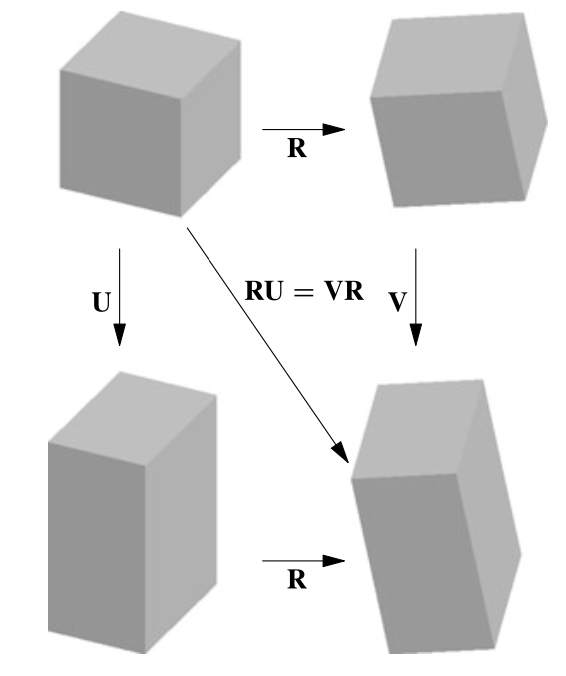
\includegraphics[width=0.5\linewidth]{images/def2}\ \ }
\end{Figure}

\rule{0.31\textwidth}{0.2pt}
\smallskip

\textbf{Cauchy-Green tensors.} They are defined as
\begin{align*}
\text{left}\quad B&=FF^T=V^2 \\
\text{right}\quad C&=F^TF=U^2
\end{align*}

Obv $B,C\in\text{Sym}^+$ and 
\begin{Figure}
    \center{
    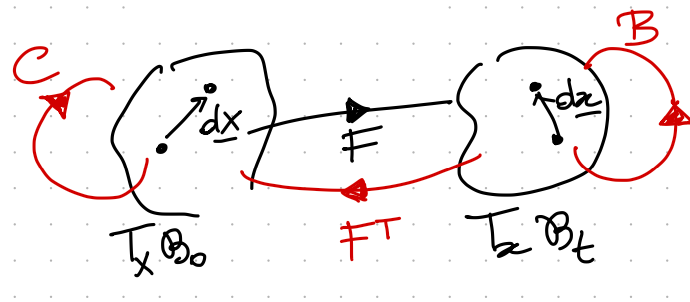
\includegraphics[width=0.7\linewidth]{images/def3}\ \ }
\end{Figure}

\rule{0.31\textwidth}{0.2pt}
\smallskip

\textbf{Motion.} Simply, it's $\underline{x}=\chi(\underline{X},t)=\underline{x}(\underline{X},t)$, so
\begin{equation*}
F(\underline{X},t)=\nabla_{\!\! _X} \underline{x}(\underline{X},t)
\end{equation*}

\vspace{-1em}

\rule{0.31\textwidth}{0.2pt}
\smallskip

\textbf{Material and spatial gradient.} $\phi=\phi(\underline{x},t)$ spatial field, its spatial gradient is
\begin{equation*}
\nabla_{\!\!_x} \phi=\frac{\partial \phi}{\partial \underline{x}}
\end{equation*}

Instead, its material gradient is 
\begin{equation*}
\nabla_{\!\!_X} \phi_m=\frac{\partial \phi_m}{\partial \underline{X}}=\frac{\partial \phi_m}{\partial \underline{x}}\,\frac{\partial \underline{x}}{\partial \underline{X}}=\left( \nabla_{\!\!_x} \phi \right)_m \cdot F
\end{equation*}

formally, just $\boxed{\nabla_{\!\!_X} \phi=\nabla_{\!\!_x} \phi\cdot F}$

\rule{0.31\textwidth}{0.2pt}
\smallskip

\newcolumn

\textbf{Velocity and acceleration.} They are
\begin{equation*}
\dot{\underline{x}}(\underline{X},t)=\frac{\partial\, \underline{x}(\underline{X},t)}{\partial t} \quad  \ddot{\underline{x}}(\underline{X},t)=\frac{\partial^2 \underline{x}(\underline{X},t)}{\partial t^2}
\end{equation*}

and $\underline{v},\underline{a}$ are the equivalent spatial representation.

\smallskip

The gradient of the material velocity is
\begin{equation*}
\nabla_{\!\!_{X}} \dot{\underline{x}}=\frac{\partial}{\partial \underline{X}} \frac{\partial\underline{x}}{\partial t}\overset{\scriptstyle\text{SW}}{=} \frac{\partial}{\partial t} \frac{\partial \underline{x}}{\partial \underline{X}}=\dot{F}
\end{equation*}

so formally, $\boxed{L:=\nabla_{\!\!x}\underline{v}=\dot{F}F^{\,\text{-}1}}$ 

\smallskip

By orthgonal decomposition for $2^{\text{nd}}$-rank tensor
\begin{equation*}
L=\frac{L+L^T}{2} +\frac{L-L^T}{2} =D+W
\end{equation*}

where $D\in\text{Sym}$ is the stretching tensor and $W\in\text{Skw}$ is the spin tensor.

\vspace{-0.5em}

\rule{0.31\textwidth}{0.2pt}
\smallskip

\textbf{Material and spatial time derivative.} $\phi$ spatial field, its spatial time derivative is
\begin{equation*}
\phi'=\frac{\partial \phi}{\partial t}
\end{equation*}

Instead, its material time derivative is 
\begin{equation*}
\left(\phi_m\right)^\cdot=\left(\phi'\right)_m+\left( \nabla_{\!\!_x} \phi \right)_m \cdot \dot{\underline{x}}
\end{equation*}

formally, just $\boxed{\dot{\phi}=\phi'+\nabla_{\!\!_x} \phi \cdot \underline{v}}$

\smallskip

Using this formula with $\phi\equiv \underline{v}$ we obtain
\begin{equation*}
\boxed{\underline{a}=\underline{v}'+ \left(\nabla_{\!\!_x}\underline{v} \right) \underline{v}}
\end{equation*}

\rule{0.31\textwidth}{1pt}











